% ---------
%  Compile with "pdflatex hw0".  
% --------
%!TEX TS-program = pdflatex

\documentclass[letterpaper,11pt]{article}
\usepackage{jeffe,handout,graphicx}
\usepackage{fancyhdr}
\usepackage{comment}
\graphicspath{{./Fig/}}

\bibliographystyle{unsrt}
% ---------
% Input file uses Unicode's UTF-8 encoding
% ---------
%!TEX encoding = UTF-8 Unicode
\usepackage[T1]{fontenc}
\usepackage[utf8]{inputenc}

% ---------
%  The next several lines (up to the line of =='s) change the default text
%  and math fonts and make a few other minor cosmetic changes.  If you get
%  any error messages related to these packages, just comment them out.
%         -- Jeff
% --------
\usepackage[charter]{mathdesign}
 \def\sfdefault{fvs}
 \def\ttdefault{fvm}
 \SetMathAlphabet{\mathsf}{bold}{\encodingdefault}{\sfdefault}{b}{\updefault}
 \SetMathAlphabet{\mathtt}{bold}{\encodingdefault}{\ttdefault}{b}{\updefault}
 \SetMathAlphabet{\mathsf}{normal}{\encodingdefault}{\sfdefault}{\mddefault}{\updefault}
 \SetMathAlphabet{\mathtt}{normal}{\encodingdefault}{\ttdefault}{\mddefault}{\updefault}
 \usepackage{microtype}
% ---------
%  End of cosmetics.
% --------

\newcommand{\name}{Zigang Xiao (zxiao2), Yuelin Du (du6)} 
\newcommand{\hwnumber}{1}                % fill homework count
\newcounter{probid}
\newtheorem{definition}{Definition}
\newcommand{\hdr}[2]{
   \newpage\setcounter{page}{1}       % reset page counter
   \lhead{\fancyplain{}{\textbf{#1}}}
   \rhead{\fancyplain{}{\textbf{#2}}}
   \cfoot{\fancyplain{}{\thepage}}
}

\newcommand{\saystmt}{
\item[($\bullet$)] \EMPH{I understand the course policies.}
}

\newcommand{\newprob}{
\hdr{CS 573 HW\hwnumber}{\name{} HW\hwnumber{} \#\arabic{probid}}
\stepcounter{probid}
\item
}

% =========================================================
\begin{document}
\pagestyle{fancy}
\fancyhf{}
\small\sf	% typeset excetps from problems in a different, smaller font

\begin{enumerate}
% ---------------------------------------------------------
\newprob

\newcommand{\EGI}{\textrm{\textsc{EvenGraphIsomorphism}}}
\newcommand{\GI}{\textrm{\textsc{GraphIsomorphism}}}
\newcommand{\SI}{\textrm{\textsc{SubgraphIsomorphism}}}
\begin{enumerate}
\saystmt
\item \label{EGItoGI}
  Describre a polynomial-time reduction from \EGI to \GI{}.

\begin{solution}
  \EGI{} is a special case of \GI{}. We can perform an identical
  reduction from \EGI{} to \GI{}. That is, given two graphs $G$ and $H$ in
  which every vertex has even degree, let $G'=G$ and $H'=H$. Then, $G$ and
  $H$ are isomorphic if and only if $G'$ and $H'$ are isomorphic.
  This copy just takes $O(n)$ time and is thus polynomial.
\end{solution}

\item 
  Describre a polynomial-time reduction from \GI{} to \EGI{}.
\begin{solution}
  Given a graph $G$, we can transform it into an even graph by adding a 
  dummy vertex between each pair of vertices that share an edge, and connect
  this vertex with the two vertices, respectively. For example, 
  we can transform the graphs $G$ and $H$ as follows:

  \begin{center}
    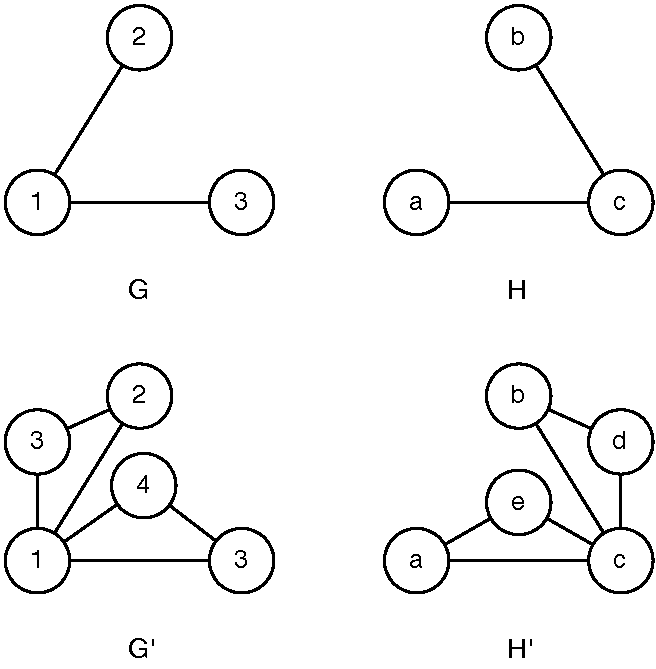
\includegraphics[width=.4\textwidth]{evengraph}\\
  \end{center}

  From graph $G$ to $G'$, vertices 3 and 4 are added between vertices 1 and 2,
  1 and 3, respectively.  From graph $H$ to $H'$, vertices $d$ and $e$ are
  added between vertices $b$ and $c$, $c$ and $a$, respectively.  The degree of
  vertices are all even after the transformation.  Given a relabeling of $G$
  and $H$, we can get a relabeling for $G'$ and $H'$ by appending the labeling
  of the added vertices to the original labeling.  Given a relabeling of the
  even graphs, we can get a relabeling for the original graphs by ignoring the
  dummy vertices. Hence, $G$ and $H$ are isomorphic if and only if $G'$ and
  $H'$ are isomorphic. There are $O(|V|)$ edges to process and thus the 
  reduction is polynomial-time.
\end{solution}

\item
  Describre a polynomial-time reduction from \GI{} to \SI{}.

\begin{solution}
  \GI{} is a speicial case of \SI{}. Given $G$ and $H$, if they do not have the
  same number of vertices and edges, of course they are not the isomorphic.  We
  perform an identical reduction from \GI{} to \SI{}.  Let $G'=G$ and $H'=H$.
  Then, $G$ and $H$ are isomorphic if and only if $G'$ and $H'$ are isomorphic
  and have the same number of vertices and edges. This reduction is polynomial
  as shown before.
\end{solution}

\item 
  Prove that \SI{} is NP-complete.

\begin{solution}
  We prove \SI{} is NP-hard by showing a polynomial time reduction from Hamiltonian Cycle problem.

\begin{proof}
  Given a graph $H$, we generate another graph $G$ such that $G$ is a cycle and
  has the same number of vertices as $H$. If $G$ is isomorphic to a subgraph of $H$, 
  then $H$ has a hamiltonian cycle, which is just the isomorphic subgraph. 
  Conversely, if $H$ has a hamiltonian cycle, $G$ will be isomorphic to the cycle,
  which is a subgraph of $H$. This transformation takes $O(n)$ time. 
  Hence, \SI{} is NP-hard. 
\end{proof}

Given a proof of subgraph isomorphism, i.e., a relabeling of a graph $G$ to a
subgraph of $H$, we apply the relabeling to $H$. Suppose we use adjacency list
to represent the graph, then we need at most $O(n^2)$ time to check if the
relabeling is correct.  The check can be done in polynomial time and thus \SI{}
in NP\@. In conclusion, \SI{} is NP-complete.

\end{solution}

\item
  What can you conclude about the NP-hardness of \GI? Justify your answer.

\begin{solution}
  I have no idea~\cite{graphisomorphism}.
\end{solution}
\end{enumerate}

\begin{thebibliography}{1} 
\bibitem{graphisomorphism}
  Wiki page on graph isomorphism.
  \newblock
  \url{http://en.wikipedia.org/wiki/Graph_isomorphism_problem#Complexity_class_GI}.
\end{thebibliography}


% ---------------------------------------------------------
\newprob

\begin{enumerate}
\saystmt
\item
  Describe and analyze a polynomial-time algorithm that computes an actual
  proper 3-coloring of a given graph $G$, or correctly reports that no such
  coloring exists, using this magic black box as a subroutine.

\begin{solution}
  For illustration purpose we name the three color as $r$, $g$, and $b$. 
  Given $G=(V,E)$, we first add a complete graph $K_3$ to $G$ as a `color
  gadget'.  Then, the three vertices in the gadget must be colored differently
  using the three colors. Without loss of generality we fix their colors and
  use the color as their names.  We denote the augmented graph as $G^+$.   At
  first we use the black box to test if the original graph is 3-colorable.
  Return \textrm{\textsc{None}} if answer is $NO$. Next, for every vertices $u$
  in $V$, we try to link them with either pair of the vertices in the gadget
  and form a new graph, such that when performing coloring, $u$ has to have the
  same color as the unselected vertex in the gadget. We then use the magic
  black box to test whether the new graph is 3-colorable.  If $YES$ then we
  output the color of the vertex that is not connected to $u$ in the gadget,
  and add these two edges into $G^+$.  Otherwise, we continue to test another
  pair. Let $V(G)$ denote the vertex set of $G$ and $E(G)$ the edge set of $G$.
  The black box is refered as $\mathsc{3Colorable($G$)}$.
  The pseudo code is given as follows:

\begin{center}\small
\begin{algorithm}
\textul{$\mathsc{3Coloring}(G)$:}\+
\\  if $\mathsc{3Colorable($G$)}$ is $\mathsc{No}$\+
\\    return $\mathsc{None}$\-
\\  $G^+ \gets (V\cup\{r, g, b\}, E\cup\{(r,g),(r,b),(g,b)\})$ 
\\  for each $u$ in $V$\+
\\    for each $v$ in $\{r,g,b\}$\+
\\      $E' \gets E(G^+) \cup \{(u,r), (u,g), (u,b)\} / \{(u,v)\}$ 
\\      $H \gets (V(G^+), E')$
\\      if $\mathsc{3Colorable($H$)}$ is $\mathsc{Yes}$ \+
\\        color[$u$] $\gets$ color of $v$
\\        $G^+ \gets H$
\\        break\-\-\-
\\  return color 
\end{algorithm}
\end{center}

 An illustration is given as follows:

\begin{center}
  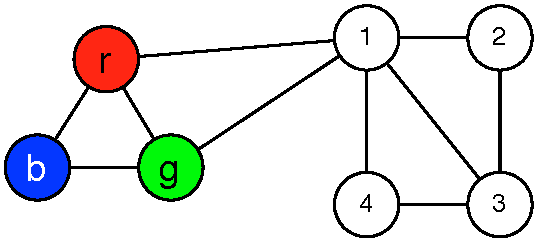
\includegraphics[width=.3\textwidth]{coloring}\\
\end{center}

At first vertex 1 is connected to $r$ and $g$, which means it should be
colored to blue. Use the black box to test whether the new graph is
3-colorable.

\textbf{Correctness:} At each step of connecting a vertex to a pair of vertices
in the color gadget, the color of this particular vertex is fixed. Suppose a
proof of the problem is a permutation of colors $rgbbgrrb\cdots$, essentially
we are guessing the prefix of the proof, and verify it using the black box.
This gurantees a correct answer.

\textbf{Complexity:} 
Let the time complexity of black box subroutine be $f(n)$.  At first there is
call to the subroutine and some constant-time operations.  The algorithm
contains a for loop that will traverse the vertex set of given graph $G$.
Inside the for loop at most three steps will be performed, which contains a
call to the subroutine and some constant time operations.  The time complexity
will be $O(f(n))+\alpha+3n(\beta+O(f(n)))$, where $\alpha$ and $\beta$ are some
constants.  Hence, this algorithm is polynomial-time.
\end{solution}

\end{enumerate}

% ---------------------------------------------------------
\newprob

\begin{enumerate}
\saystmt
\item
  Prove that deciding whether a graph has a heavy Hamiltonian cycle is
  NP-complete.

\begin{solution}
  We reduce from Hamiltonian Path problem. Given a graph $G=(V,E)$, we add two
  vertices $s$ and $t$ that connects all $v$ in $V$, respectively. Also $s$ and
  $t$ is connected.  Then we get a graph $G'=(V',E')$, where $V'=V\cup \{s,t\}$
  and $E'=E\cup \{(s,t)\} \cup \{(s,v), (t,v) \ |\  v\in V\}$.  We assign a
  weight $|E|+2|V|$ to $(s,t)$, and 1 to all other edges.  An illustration is
  given as follows: 

  \begin{center}
    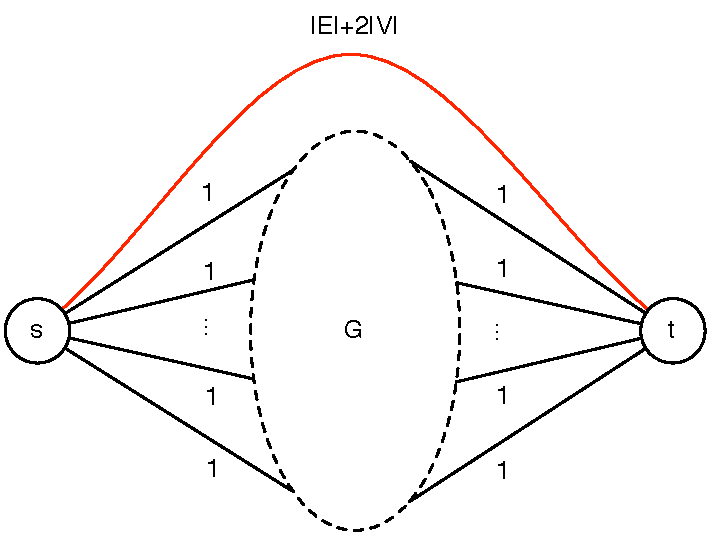
\includegraphics[width=.5\textwidth]{hamcycle}\\
  \end{center}
  
  \textbf{Correctness:}
  We claim that $G$ has a Hamiltonian Path if and only if $G'$ has a heavy
  Hamiltonian Cycle.  The total weight of the graph is
  $|E|+2|V|+2|V|+|E|=4|V|+2|E|$.  Hence, the weight of $(s,t)$ dominates the
  weight of the possible Heavy Hamiltonian Cycle, i.e., $(s,t)$ must be
  included in a Heavy Hamiltonian Cycle.  $s$ can only be visited once, $(s,t)$
  is already used and there will be another edge $(s, v)$ included in the cycle
  where $v \in E$.  Similary for $t$. Because $s$ and $t$ are connected to
  every vertex in $E$ respectively, the Hamiltonian Cycle can be closed if and
  only there is a Hamiltonian Path in $E$. 
  
  \textbf{Complexity:}
  We only need linear time to create two vertices and connect them with the
  exisiting vertices. Hence the reduction takes polynomial time.

  Heavy Hamiltonian cycle problem is in NP\@, because we can easily verify the
  answer by using a depth or breadth-first search to compute the total weight,
  and follow the cycle to compute the weight of the cycle. This takes linear
  time. In conclusion, Heavy Hamiltonian cycle problem is NP-complete.
\end{solution}

\end{enumerate}

% ---------------------------------------------------------
\newprob

\begin{enumerate}
\saystmt
\item
  Prove that it is NP-hard to determine, given an initial configuration of red and blue stones, whether the puzzle can be solved.

\begin{solution}
  We reduce from 3SAT to this decision problem. Given a instance of 3SAT, let
  $n$ be the number of clauses, and $m$ be the number of different variables.
  We designate each variable to a different column.  For each clause, we create
  a row for it in the game, where each column in that row corresponds to a
  literal. In each row, a blue stone is placed if the literal is a variable, or
  a red stone if it is its negation. For the variables that are not included in
  the clause, we simply leave the corresponding squares to be empty. Finally a
  $n\times m$ grids of squares will be constructed.
  For example, given a formula 
  $(a \vee b \vee c) \wedge (b\vee \bar{c} \vee \bar{d}) \wedge (\bar{a} \vee c \vee d) \wedge (a \vee \bar{b} \vee \bar{d})$, 
  we can create an exact game setup as shown in the problem statement, where
  $a$, $b$, $c$, and $d$ denote column 1, 2, 3 and 4 from let to right
  respectively.  
  
  \textbf{Correctness:} The conjunctive normal form of the formula ensures the
  first condition of the game to be satisifed, because a clause is satisfied if
  and only if at least one literal is set to true, which is equivalent to at
  least one stone is in the corresponding row.  Since contradictory literals
  are placed in the same column, the assignment is consistent, which means no
  conflicting stones will be in the same column, and satisfies the second
  condition of the game.  Hence, the boolean formula is satisfiable if and only
  if the puzzle is solvable. Thus, the reduction is correct. 

  \textbf{Complexity:} We only need linear time to perform this reduction,
  since we can allocate a column to a new variable as we go. Hence the
  reduction is polynomial-time.

  In conclusion, this decision problem is NP-hard.

\end{solution}

\end{enumerate}

% ---------------------------------------------------------
\newprob

\begin{enumerate}
\saystmt
\item
   Either describe
   a polynomial-time algorithm for XCNF-SAT or prove that it is NP-complete.

\begin{solution} 
  XCNF-SAT can be solved in polynomial time. In order to satisfy a clause, the
  binary sum of the literals inside must be 1 (mod 2), since a exclusive-or 
  clause is satisfied if and only if there is odd number of true literals.
  Hence, we can construct a system of linear equation over modulo 2. 
  For each clause, an equation will be constructed. The left hand side contains
  the sum of the variables. If a literal is the negation of some variable $x$,
  we transformed it into $x+1$ in the equation; The right hand side is 1 (mod 2).
  For example, for the clause:
  \[u \oplus v \oplus \bar{w} \oplus x\] 
  We can transform it into:
  \[u+v+w+1+x \equiv 1 \ (\textrm{mod } 2)\]  
  By using Gaussian
  Elimination method for binary arithmetic, we can solve this sytem and obtain
  the satisfying assignments.  It takes linear time to scan the boolean formula
  and construct the linear system.  Given a XCNF-SAT instance that contains $m$
  clauses and $n$ variables, Gaussian Elimination for binary arithmetic takes
  $O(mn^2)$ time~\cite{Gaussian}.  Hence, our algorithm runs in
  polynomial-time.

\end{solution}
\end{enumerate}

% =========================================================
\end{enumerate}
\begin{thebibliography}{1} 
\bibitem{Gaussian}
Wiki page on Gaussian elimination.
\newblock
\url{http://en.wikipedia.org/wiki/Gaussian_elimination#Analysis}.
\end{thebibliography}
\end{document}
